\documentclass{article}
\usepackage{amsmath,amsfonts,amssymb}
\usepackage[margin=1in]{geometry}
\usepackage{graphicx}
\usepackage{tikz}
\usetikzlibrary{arrows}
\begin{document}

\title{ELCT 432: Problem Assignment \#4}
\author{Jacob C. Vaught}
\date{9-30-2023}
\maketitle

\section*{Problem \#1[10 Points]}

We have a 300 MHz sinusoidal carrier signal frequency modulated by a sinusoid such that the maximum frequency deviation \( \Delta f = 100 \, \text{kHz} \). Find the modulation index \( \beta \) and the approximate bandwidth (i.e., Carson's rule) of the FM signal for the following three values of the modulating signal frequency:

\begin{itemize}
  \item[(a)] \( f_m = 1 \, \text{kHz} \)
  \item[(b)] \( f_m = 100 \, \text{kHz} \)
  \item[(c)] \( f_m = 500 \, \text{kHz} \)
\end{itemize}

\subsection*{Solutions}

\subsubsection*{Modulation Index \( \beta \)}

The modulation index \( \beta \) is defined as:
\[
\beta = \frac{\Delta f}{f_m}
\]

\textbf{(a) \( f_m = 1 \, \text{kHz} \)}
\[
\beta = \frac{100 \, \text{kHz}}{1 \, \text{kHz}} = 100
\]

\textbf{(b) \( f_m = 100 \, \text{kHz} \)}
\[
\beta = \frac{100 \, \text{kHz}}{100 \, \text{kHz}} = 1
\]

\textbf{(c) \( f_m = 500 \, \text{kHz} \)}
\[
\beta = \frac{100 \, \text{kHz}}{500 \, \text{kHz}} = 0.2
\]

\subsubsection*{Approximate Bandwidth (Carson's Rule)}

Carson's rule estimates the bandwidth \( B \) as:
\[
B \approx 2(\Delta f + f_m)
\]

\textbf{(a) \( f_m = 1 \, \text{kHz} \)}
\[
B \approx 2(100 \, \text{kHz} + 1 \, \text{kHz}) = 202 \, \text{kHz}
\]

\textbf{(b) \( f_m = 100 \, \text{kHz} \)}
\[
B \approx 2(100 \, \text{kHz} + 100 \, \text{kHz}) = 400 \, \text{kHz}
\]

\textbf{(c) \( f_m = 500 \, \text{kHz} \)}
\[
B \approx 2(100 \, \text{kHz} + 500 \, \text{kHz}) = 1.2 \, \text{MHz}
\]

\newpage
\section*{Problem \#2[10 Points]}
Given a message signal \( m(t) = 19 \cos(2\pi \times 16000 t + 7) \), find the bandwidth of the modulated signal for a carrier wave with amplitude \( 2 \) and frequency \( 1.1 \, \text{GHz} \) for the following cases:

\begin{enumerate}
  \item Conventional AM with \( k_a = 0.432025358 \)
  \item DSB-SC
  \item FM with \( k_f = 5000 \, \text{Hz/v} \)
\end{enumerate}

\subsection*{Solutions}

\subsubsection*{Conventional AM}

For Conventional Amplitude Modulation (AM), the bandwidth is essentially double the highest frequency component of the modulating signal.

\[
\text{Bandwidth for AM} = 2 \times f_m = 2 \times 16000 = 32000 \, \text{Hz} = 32 \, \text{kHz}
\]

\subsubsection*{DSB-SC}

For Double-Sideband Suppressed Carrier (DSB-SC), the bandwidth is the same as that for Conventional AM.

\[
\text{Bandwidth for DSB-SC} = 2 \times f_m = 2 \times 16000 = 32000 \, \text{Hz} = 32 \, \text{kHz}
\]

\subsubsection*{FM}

For Frequency Modulation (FM), we use Carson's rule to approximate the bandwidth:

\[
\text{Bandwidth for FM} \approx 2 \left( f_m + \Delta f \right)
\]

where \( \Delta f = k_f \times A_m \), \( A_m = 19 \), and \( k_f = 5000 \, \text{Hz/v} \).

\[
\Delta f = 5000 \times 19 = 95000 \, \text{Hz} = 95 \, \text{kHz}
\]
\[
\text{Bandwidth for FM} \approx 2 \left( 16000 + 95000 \right) = 222000 \, \text{Hz} = 222 \, \text{kHz}
\]

\newpage
\section*{Problem \#3[10 Points]}
Given an FM signal \( s_{FM}(t) = \cos\left(2\pi f_c t + \beta_f \sin (2\pi 10 t)\right) \) with \( \beta_f = 5 \), find the coefficient of the FM spectrum at \( f_c + 20 \).

\subsection*{Solutions}

The spectrum of an FM signal can be generally expressed as:

\[
S(f) = \sum_{n=-\infty}^{\infty} J_n(\beta_f) \cdot \delta(f - f_c \pm n f_m)
\]
\newline
We are interested in finding the coefficient at \( f_c + 20 \). The value of \( f_m \) is \( 10 \) and therefore \( n \) should be \( 2 \) for \( f_c + n f_m = f_c + 20 \).
\newline\newline
The coefficient at \( f_c + 20 \) will therefore be \( J_2(5) \).


\newpage
\section*{Problem \#4[20 Points]}
Given a message signal \( m(t) = A_m \sin(2\pi f_m t) \) with \( A_m = 0.5 \) and \( f_m = 128 \) Hz, a carrier frequency \( f_c = 1024 \) Hz, and amplitude \( A_c = 1 \):

\begin{enumerate}
    \item Specify \( s(t) \) for AM with 30\% modulation. What is the bandwidth of the signal?
    \item Repeat (a) for DSB-AM.
    \item Repeat for FM with \( k_f = 400 \) Hz. Also, determine the peak frequency deviation.
\end{enumerate}

\subsection*{Solutions}

\subsubsection*{(a) Amplitude Modulation (AM)}
The equation for an AM signal with modulation index \( \mu \) is:
\[
s(t) = A_c (1 + \mu m(t)) \cos(2\pi f_c t)
\]
Here, \( \mu = 0.3 \). Therefore,
\[
s(t) = (1 + 0.3 \times 0.5 \sin(2\pi \times 128 t)) \cos(2\pi \times 1024 t)
\]
The bandwidth of the AM signal will be \( 2f_m = 2 \times 128 = 256 \) Hz.

\subsubsection*{(b) Double-Sideband Amplitude Modulation (DSB-AM)}
The equation for a DSB-AM signal is similar to AM without the carrier component:
\[
s(t) = A_m A_c \sin(2\pi f_m t) \cos(2\pi f_c t)
\]
Therefore,
\[
s(t) = 0.5 \times 1 \sin(2\pi \times 128 t) \cos(2\pi \times 1024 t)
\]
The bandwidth of the DSB-AM signal is also \( 2f_m = 256 \) Hz.

\subsubsection*{(c) Frequency Modulation (FM)}
The equation for an FM signal is:
\[
s(t) = A_c \cos(2\pi f_c t + k_f \int m(t) \, dt)
\]
Here \( k_f = 400 \) Hz. The integral of \( m(t) = 0.5 \sin(2\pi \times 128 t) \) is \( -\frac{0.5}{2\pi \times 128} \cos(2\pi \times 128 t) \). Therefore,
\[
s(t) = \cos\left(2\pi \times 1024 t - 400 \times \frac{0.5}{2\pi \times 128} \cos(2\pi \times 128 t)\right)
\]
The peak frequency deviation \( \Delta f \) is \( k_f \times A_m = 400 \times 0.5 = 200 \) Hz.

\newpage
\section*{Problem \#5[20 Points]}

Consider a carrier signal with amplitude \( A_c = 1 \) and \( f_c = 100 \) MHz. The message signal is \( m(t) = \sin(2\pi \times 2000 t) \). 

\begin{enumerate}
    \item What is the signal bandwidth for:
    \begin{enumerate}
        \item Conventional AM with \( a = 0.5 \)?
        \item DSB-SC AM?
        \item FM with \( k_f = 4000 \) Hz?
    \end{enumerate}
    \item What are the expressions for the transmitted signals in each case in part (a)?
    \item What is the transmitted power for each signal in part (a)?
\end{enumerate}

\subsection*{Solutions}

\subsubsection*{(a) Signal Bandwidth}

\begin{enumerate}
    \item \textbf{Conventional AM}: The bandwidth for AM is \(2f_m\), where \(f_m = 2000 \) Hz. Hence, \(BW = 2 \times 2000 = 4000 \) Hz.
    \item \textbf{DSB-SC AM}: The bandwidth is the same as for conventional AM, \(BW = 4000 \) Hz.
    \item \textbf{FM}: The modulation index \( \beta = \frac{\Delta f}{f_m} \), where \( \Delta f = k_f \times A_m \) and \( A_m = 1 \). So, \( \Delta f = 4000 \) Hz, and \( \beta = \frac{4000}{2000} = 2 \). Using Carson's rule, \( BW = 2(f_m + \Delta f) = 2(2000 + 4000) = 12000 \) Hz.
\end{enumerate}

\subsubsection*{(b) Transmitted Signals}

\begin{enumerate}
    \item \textbf{Conventional AM}: \( s(t) = (1 + 0.5 \sin(2\pi \times 2000 t)) \cos(2\pi \times 100 \times 10^6 t) \)
    \item \textbf{DSB-SC AM}: \( s(t) = \sin(2\pi \times 2000 t) \cos(2\pi \times 100 \times 10^6 t) \)
    \item \textbf{FM}: \( s(t) = \cos(2\pi \times 100 \times 10^6 t + 2\pi\times4000 \int \sin(2\pi \times 2000 t) \, dt) \)
\end{enumerate}

\subsubsection*{(c) Transmitted Power}

\begin{enumerate}
    \item \textbf{Conventional AM}: \( P = \frac{A_c^2}{2} (1 + \frac{a^2}{2}) = \frac{1}{2}(1 + \frac{0.25}{2}) = 0.5625 \) W
    \item \textbf{DSB-SC AM}: \( P = \frac{A_c^2 A_m^2}{4} = \frac{1 \times 1}{4} = 0.25 \) W
    \item \textbf{FM}: The power of an FM signal is just the power of the carrier, \( P = \frac{A_c^2}{2} = \frac{1}{2} \) W
\end{enumerate}


\newpage
\section*{Problem \#6[20 Points]}

Assume that the signal is \( u(t) = A_c \cos(2\pi f_c t + 100 \sin(t)) \). 

\begin{enumerate}
    \item What is the corresponding instantaneous frequency?
    \item What is the maximum frequency deviation around the carrier frequency \( f_c \)?
\end{enumerate}

\subsection*{Solutions}

\subsubsection*{(a) Instantaneous Frequency}

The instantaneous phase of \( u(t) \) is given as \( \phi(t) = 2\pi f_c t + 100 \sin(t) \). Taking the derivative with respect to \( t \) we get:

\[
\frac{d\phi(t)}{dt} = 2\pi f_c + 100 \cos(t)
\]

The instantaneous angular frequency \( \omega_i(t) \) is \( \frac{d\phi(t)}{dt} \), and the instantaneous frequency \( f_i(t) \) is \( \frac{\omega_i(t)}{2\pi} \):

\[
f_i(t) = f_c + \frac{100 \cos(t)}{2\pi}
\]

\subsubsection*{(b) Maximum Frequency Deviation}

The maximum frequency deviation \( \Delta f \) can be determined from the term affecting the instantaneous frequency, \( 100 \cos(t) / 2\pi \). The maximum deviation occurs when \( \cos(t) = \pm 1 \):

\[
\Delta f = \frac{100}{2\pi}
\]

Thus, the maximum frequency deviation \( \Delta f \) is \( \frac{100}{2\pi} \) Hz.



\newpage
\section*{Problem \#7[10 Points]}

For \( x(t) = B \, \text{sinc}(Bt) \cos(2\pi f_c t) \) where \( f_c \gg 1 \) and \( B = 20 \, \text{MHz} \), determine:

\begin{itemize}
  \item[(a)] Express the Fourier transform (FT) of \( x(t) \).
  \item[(b)] Draw the spectrum (only \( |X(f)| \)) and show the values on both \( x \)- and \( y \)-axes.
\end{itemize}

\section*{Solutions}

\subsection*{Fourier Transform of \( x(t) \)}

We are given the time-domain signal \( x(t) \) as:

\[
x(t) = B \, \text{sinc}(Bt) \cos(2\pi f_c t)
\]

To find its Fourier Transform \( X(f) \), we will utilize two main properties of the Fourier Transform: modulation and convolution.

\subsubsection*{Step 1: Fourier Transform of the sinc Function}

First, we consider the Fourier Transform of the sinc function \( \text{sinc}(Bt) \). By standard Fourier Transform tables, we know that:

\[
\mathcal{F}\{\text{sinc}(Bt)\} = \text{rect}\left(\frac{f}{B}\right)
\]

Here \( \text{rect}(x) \) is the rectangular function, defined as:

\[
\text{rect}(x) = 
\begin{cases} 
1, & \text{if } |x| < \frac{1}{2} \\
0, & \text{otherwise}
\end{cases}
\]

This rectangular function in the frequency domain has a width of \( 2B \).

\subsubsection*{Step 2: Modulation}

Multiplying \( \text{sinc}(Bt) \) by \( \cos(2\pi f_c t) \) in the time domain corresponds to frequency modulation in the frequency domain. This results in the creation of sidebands located at \( f_c \) and \( -f_c \).

The Fourier Transform \( X(f) \) can be mathematically represented as:

\[
X(f) = \frac{B}{2} \left( \text{rect}\left(\frac{f - f_c}{B}\right) + \text{rect}\left(\frac{f + f_c}{B}\right) \right)
\]

In this formula, \( \text{rect}\left(\frac{f - f_c}{B}\right) \) signifies the part of the spectrum that has been shifted to \( f_c \), and \( \text{rect}\left(\frac{f + f_c}{B}\right) \) represents the part shifted to \( -f_c \).

The division by 2 occurs because the original spectrum of \( \text{sinc}(Bt) \) is effectively being split between the two sidebands, each receiving half of the total spectral energy.

\newpage
\subsection*{Spectrum \( |X(f)| \)}

\subsubsection*{Drawing the Spectrum}
I am unsure if there needs to be a division by $2\pi$ so I included both options. \newline\newline
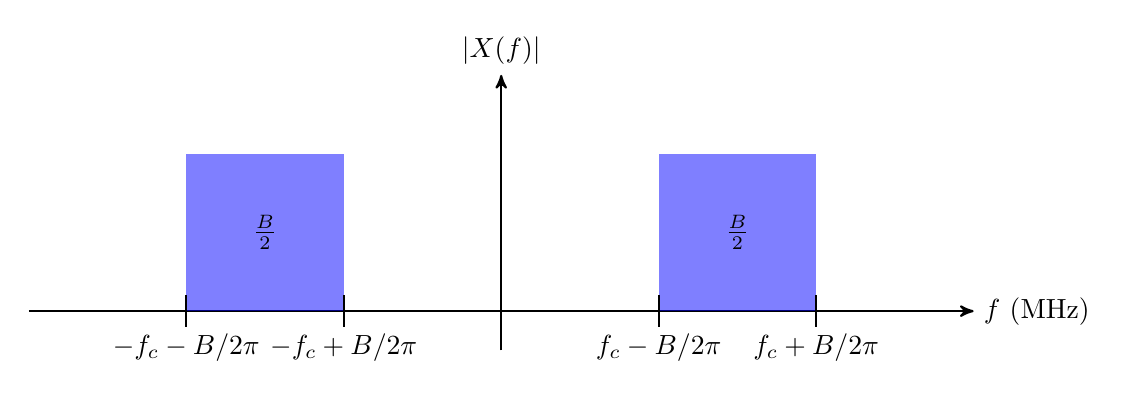
\begin{tikzpicture}[>=stealth']
    % Draw x-axis and y-axis
    \draw[thick,->] (-6,0) -- (6,0) node[right] { \( f \) (MHz)};
    \draw[thick,->] (0,-0.5) -- (0,3) node[above] { \( |X(f)| \) };

    % Draw rectangles for frequency components
    \fill[blue,opacity=0.5] (-4,0) rectangle (-2,2);
    \fill[blue,opacity=0.5] (2,0) rectangle (4,2);

    % Label frequency components
    \node at (-3,1) { \( \frac{B}{2} \) };
    \node at (3,1) { \( \frac{B}{2} \) };

    % Label frequency values
    \draw[thick] (-2,-0.2) -- (-2,0.2) node[below=10pt] { \( -f_c + B/2\pi \) };
    \draw[thick] (-4,-0.2) -- (-4,0.2) node[below=10pt] { \( -f_c - B/2\pi \) };
    \draw[thick] (2,-0.2) -- (2,0.2) node[below=10pt] { \( f_c - B/2\pi \) };
    \draw[thick] (4,-0.2) -- (4,0.2) node[below=10pt] { \( f_c + B/2\pi \) };
\end{tikzpicture}
\newline
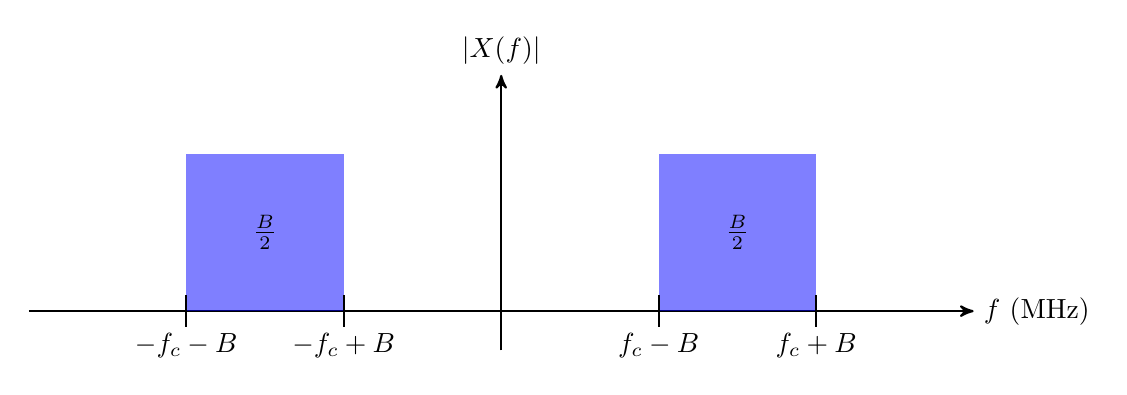
\begin{tikzpicture}[>=stealth']
    % Draw x-axis and y-axis
    \draw[thick,->] (-6,0) -- (6,0) node[right] { \( f \) (MHz)};
    \draw[thick,->] (0,-0.5) -- (0,3) node[above] { \( |X(f)| \) };

    % Draw rectangles for frequency components
    \fill[blue,opacity=0.5] (-4,0) rectangle (-2,2);
    \fill[blue,opacity=0.5] (2,0) rectangle (4,2);

    % Label frequency components
    \node at (-3,1) { \( \frac{B}{2} \) };
    \node at (3,1) { \( \frac{B}{2} \) };

    % Label frequency values
    \draw[thick] (-2,-0.2) -- (-2,0.2) node[below=10pt] { \( -f_c + B \) };
    \draw[thick] (-4,-0.2) -- (-4,0.2) node[below=10pt] { \( -f_c - B \) };
    \draw[thick] (2,-0.2) -- (2,0.2) node[below=10pt] { \( f_c - B \) };
    \draw[thick] (4,-0.2) -- (4,0.2) node[below=10pt] { \( f_c + B \) };
\end{tikzpicture}

\end{document}
